\documentclass[11pt]{exam}
\usepackage{epsfig}
\usepackage{graphicx}
\usepackage{hyperref}
\usepackage{enumitem}
\usepackage[centertags]{amsmath}
\usepackage{amssymb}
\usepackage{amsthm}
\usepackage[all]{xy}
\usepackage{newlfont}
\usepackage{bm,mathtools}
\usepackage{xcolor}
\usepackage{verbatim}
\usepackage{subfig}
\usepackage{cleveref}
\usepackage{listings}

\graphicspath{{./media/}}

\begin{document}
\centerline{\Large \sc EEL 6878 Modeling and Artificial Intelligence (2026 Sp)}
\centerline{\Large \sc Homework Assignment}
\pagestyle{empty}

\hrulefill

\vspace{2cm}

{\Large \sc Name:}

\vspace{2cm}

{\Large \sc Student ID:}

\vspace{6cm}

\begin{itemize}
  \item Reasoning and work must be shown to gain partial/full credit.
  \item Please include the cover-page on your homework PDF with your name and student ID.
        Failure to do so is considered bad citizenship.
  \item The packages that you may need include \texttt{networkx}, \texttt{matplotlib},
        and \texttt{numpy}.
  \item For questions requiring code, submit both your code (as a \texttt{.py} or
        \texttt{.ipynb} file) and the resulting figures.
  \item Submit your written answers and figures as a single PDF. Include Python code
        as an appendix or provide a link to a GitHub repository. All sections must be
        clearly labeled and all figures must have captions.
\end{itemize}

\clearpage

\begin{questions}

%%------------------------------------------------------------
%% Q1 — 15 pts
%%------------------------------------------------------------
\question[15]{\bf Algebra of Graphs}

Considering the undirected graph in the figure:
\begin{center}
  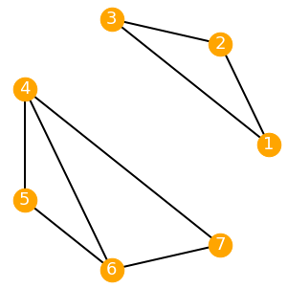
\includegraphics[width=0.3\linewidth]{homework_graph.png}
\end{center}

\begin{parts}
  \part Write the adjacency, oriented incidence, and Laplacian matrices for the graph.
  \part Show that there exist two linearly independent vectors in the null space of the
        Laplacian and explain why that is the case.
\end{parts}

%%------------------------------------------------------------
%% Q2 — 25 pts
%%------------------------------------------------------------
\question[25]{\bf Graphs with Circular Symmetry}

Consider an undirected graph with circular symmetry, i.e.,
${\cal G}=({\cal V}, {\cal E})$ such that:
\[
  {\cal V}=\{0,1,\ldots, N-1\} \qquad \text{and}\qquad
  {\cal E} = \{(u,v) \mid v=((u+i)\bmod N),\ \forall\ i\in \mathcal{I}\}
\]
For example, suppose $\mathcal{I}=\{1,2\}$ and $N>4$, then:
\begin{itemize}
  \item $(0,1)$ and $(0,2)$ are in the set since for $u=0$ and $i=1,2$,
        $((u+i)\bmod N)=i$.
  \item $(N-1,0)$ and $(N-2,0)$ are in it: for $u=N-1$ and $i=1$,
        $((N-1+1)\bmod N)=0$, and for $u=N-2$ and $i=2$,
        $((N-2+2)\bmod N)=0$.
\end{itemize}

\begin{parts}
  \part Assume $N=5$ and $\mathcal{I} = \{1\}$. Write the edge set and draw the graph.
  \part Validate numerically what is shown in lecture regarding the eigenvectors and
        eigenvalues of the Laplacian for graphs with circular symmetry.
  \part Plot the Fiedler eigenvalue\footnote{The Fiedler eigenvalue is the second
        smallest eigenvalue of the Laplacian.} for this type of graph as a function of
        $N = 5$ up to $50$ with step $5$, and explain the trend.
  \part Suppose you can add one extra edge to the graph for $N=10$. Since you have
        circular symmetry, you can explore all possible trends by adding an extra
        neighbor to node $0$. Explore numerically the trend of the Fiedler eigenvalue
        as you test the different possible options for the extra neighbor.
\end{parts}

%%------------------------------------------------------------
%% Q3 — 10 pts
%%------------------------------------------------------------
\question[10]{\bf Spectral Clustering on the Karate Club Graph}~{\it (Python/NetworkX)}

The Zachary's Karate Club graph is available directly via NetworkX
(\url{https://networkx.org/documentation/stable/reference/generated/networkx.generators.social.karate_club_graph.html}).
Load it with \texttt{networkx.karate\_club\_graph()} and partition it using the
spectral clustering algorithm into:
\begin{parts}
  \part Two communities.
  \part Three communities.
\end{parts}
For each case, plot the graph with nodes colored by community assignment and briefly
discuss the quality of the partition.

%%------------------------------------------------------------
%% Q4 — 10 pts
%%------------------------------------------------------------
\question[10]{\bf Harry Potter Network --- Data Preparation and Overview}%
~{\it (Python/NetworkX)}

This question and the two that follow apply network analysis to the Harry Potter
series. The dataset is a signed undirected graph covering the entire series,
available at \url{https://github.com/efekarakus/potter-network} and included in
the homework zip file. It contains two files:
\begin{itemize}
  \item \texttt{characters.csv} --- a list of 65 Harry Potter characters with
        biographical information.
  \item \texttt{relations.csv} --- a list of undirected relations between characters,
        where the \texttt{type} field indicates allies (\texttt{+}) or
        enemies (\texttt{-}).
\end{itemize}
Interactions are identified based on co-mentions within close proximity in the
text, signifying direct\footnote{Not to be confused with a directed edge.}
interactions between characters. Load the data as follows:
\begin{lstlisting}[language=Python]
import pandas as pd
import networkx as nx

chars = pd.read_csv("characters.csv")
edges = pd.read_csv("relations.csv")

G = nx.Graph()
for _, row in edges.iterrows():
    G.add_edge(row["source"], row["target"], type=row["type"])
\end{lstlisting}

\begin{parts}
  \part Load the overall series graph from \texttt{characters.csv} and
        \texttt{relations.csv} as described above.
  \part Provide a statistical summary of the graph, including: number of nodes,
        number of edges, average degree, density, and connectivity status.
        Also report the number of positive (ally) and negative (enemy) edges.
\end{parts}

%%------------------------------------------------------------
%% Q5 — 25 pts
%%------------------------------------------------------------
\question[25]{\bf Harry Potter Network --- Centrality Analysis}~{\it (Python/NetworkX)}

\begin{parts}
  \part Compute the following centrality metrics for all characters in the
        overall series graph:
        \begin{itemize}
          \item Degree Centrality
          \item Weighted Degree Centrality
          \item Betweenness Centrality
          \item Closeness Centrality
          \item Eigenvector Centrality
          \item PageRank
        \end{itemize}
  \part Identify the top 10 characters based on each centrality measure.
        \textbf{Visualize and discuss} the results, emphasizing how each metric
        reflects different aspects of a character's role and narrative significance
        in the series.
  \part Highlight \textbf{at least one character} whose centrality measures
        closely align with their narrative arc and provide a detailed analysis
        of this correlation. For example, consider how a character's degree of
        connectivity or brokerage role reflects their introduction, peak
        involvement, or departure from the storyline.
\end{parts}

%%------------------------------------------------------------
%% Q6 — 15 pts
%%------------------------------------------------------------
\question[15]{\bf Harry Potter Network --- Community Detection}~{\it (Python/NetworkX)}

\begin{parts}
  \part Apply community detection algorithms (e.g., Spectral Clustering, Louvain
        Method, Girvan--Newman Algorithm) to the overall Harry Potter interaction graph.
        \textbf{Visualize the resulting community structures} such that:
        \begin{itemize}
          \item Node size is scaled by each character's \textbf{PageRank}.
          \item Label size is scaled by each character's \textbf{Betweenness
                Centrality}.
        \end{itemize}
        This visualization highlights both the prominence and the brokerage roles of
        characters within their communities.
  \part Analyze the composition and configuration of the detected communities. Discuss
        the narrative significance of these groupings (e.g., characters from the same
        Hogwarts house clustering together, or alliances formed during key plot events).
        Examine how these community structures reflect the social dynamics and
        relationships throughout the series.
\end{parts}

\end{questions}

\bibliographystyle{IEEEtran}
\bibliography{ref}

\end{document}